\section{Lepton reconstruction, selection and trigger efficiencies}\label{sec:Eff}

Since the lepton reconstruction, selection and trigger efficiencies can be slightly different between data and simulation events,
correction factors have to be applied to the MC to account for these differences. The efficiencies are calculated using a Tag and Probe
technique exploiting Z boson decays to a pair of electrons or muons, respectively. One of the leptons is used as tag and has to pass a
tight selection, while the second one is used as probe if the tag-probe pair combines to the Z boson mass. The total lepton efficiency
can be factorized into three components:

\begin{equation}
\epsilon_{\textnormal{total}}=\epsilon_{\textnormal{Reco}}\cdot\epsilon_{\textnormal{Id}}\cdot\epsilon_{\textnormal{HLT}}
\end{equation}

The tag and probe method is nearly the same compared to the one already used in the 2011 data analysis for this Higgs search
(\cite{CMS-AN-12-029},\cite{CMS-AN-2012-021}). Therefore, only the most important information will be discussed.

\subsection{Electron efficiencies}\label{subsec:EffEle}
In the electron case, the reconstruction efficiency $\epsilon_{\textnormal{Reco}}$ characterizes the transition from a supercluster in the
electromagnetic calorimeter to a reconstructed Particle Flow electron. The ability of a reconstructed electron to pass the offline
selection consisting of several isolation and identification criteria is given by the identification efficiency $\epsilon_{\textnormal{Id}}$.
Finally, the selected electron has to fire the high level trigger. The efficiency to fulfill the HLT requirements is parametrized as
$\epsilon_{\textnormal{HLT}}$. Both in data and MC, a single electron trigger is used at HLT level. Since the efficiency depends both on $\pt$
and $\eta$ of the electron, the measurement is binned in $\pt$ as (30, 35, 40, 45, 50, 200)\GeVc and in $\eta$ as (-2.5, -1.5, 0.0, 1.5, 2.5) of
the probe electron. All three efficiency components can be calculated both for data and MC, so that a data/MC scale factor is computed
in all cases. The resulting efficiencies and scale factors are summarized in table~\ref{tab:eleEff1} and \ref{tab:eleEff2}. Figure~\ref{fig:eleEff}
shows the data/MC scale factors for the electron reconstruction (a), identification (b) and trigger (c).

\begin{table}[htb]
\centering 
\scalebox{0.70}{
  \begin{tabular}{|c|c|c|c|c|c|c|c|c|c|}
  \hline
  $p_{\textnormal{T,min}}$ & $p_{\textnormal{T,max}}$ & $\eta_{\textnormal{min}}$ & $\eta_{\textnormal{max}}$ & $\epsilon_{\textnormal{Reco,data}}$ & $\epsilon_{\textnormal{Reco,mc}}$ & $\textnormal{SF}_{\textnormal{Reco}}$ & $\epsilon_{\textnormal{ID,data}}$ & $\epsilon_{\textnormal{ID,mc}}$ & $\textnormal{SF}_{\textnormal{ID}}$ \\
  $[\GeVc]$         & $[\GeVc]$         &                     &                     &                              &                           &                                 &                            &                          &                                \\
  \hline
  \hline
  30	& 35	& -2.5	& -1.5	& 0.983$\pm$0.005 & 0.946$\pm$0.007 & 1.039$\pm$0.010 & 0.582$\pm$0.004 & 0.576$\pm$0.013 & 1.010$\pm$0.023 \\
  30	& 35	& -1.5	& 0	& 0.990$\pm$0.003 & 0.989$\pm$0.002 & 1.001$\pm$0.003 & 0.804$\pm$0.004 & 0.809$\pm$0.006 & 0.994$\pm$0.009 \\
  30	& 35	& 0	& 1.5	& 0.991$\pm$0.006 & 0.987$\pm$0.002 & 1.004$\pm$0.006 & 0.812$\pm$0.004 & 0.813$\pm$0.006 & 0.998$\pm$0.009 \\
  30	& 35	& 1.5	& 2.5	& 0.984$\pm$0.005 & 0.953$\pm$0.007 & 1.032$\pm$0.009 & 0.582$\pm$0.066 & 0.590$\pm$0.013 & 0.987$\pm$0.113 \\
  35	& 40	& -2.5	& -1.5	& 0.984$\pm$0.003 & 0.955$\pm$0.004 & 1.030$\pm$0.006 & 0.684$\pm$0.006 & 0.690$\pm$0.005 & 0.990$\pm$0.011 \\
  35	& 40	& -1.5	& 0	& 0.998$\pm$0.001 & 0.994$\pm$0.001 & 1.003$\pm$0.001 & 0.877$\pm$0.003 & 0.881$\pm$0.004 & 0.996$\pm$0.005 \\
  35	& 40	& 0	& 1.5	& 0.997$\pm$0.001 & 0.995$\pm$0.001 & 1.002$\pm$0.001 & 0.874$\pm$0.003 & 0.883$\pm$0.004 & 0.991$\pm$0.005 \\
  35	& 40	& 1.5	& 2.5	& 0.986$\pm$0.003 & 0.969$\pm$0.004 & 1.018$\pm$0.006 & 0.700$\pm$0.007 & 0.688$\pm$0.009 & 1.018$\pm$0.017 \\
  40	& 45	& -2.5	& -1.5	& 0.991$\pm$0.002 & 0.969$\pm$0.004 & 1.023$\pm$0.004 & 0.752$\pm$0.005 & 0.735$\pm$0.008 & 1.023$\pm$0.013 \\
  40	& 45	& -1.5	& 0	& 0.999$\pm$0.001 & 0.997$\pm$0.001 & 1.001$\pm$0.001 & 0.905$\pm$0.002 & 0.907$\pm$0.003 & 0.998$\pm$0.004 \\
  40	& 45	& 0	& 1.5	& 0.998$\pm$0.001 & 0.997$\pm$0.001 & 1.000$\pm$0.001 & 0.909$\pm$0.002 & 0.903$\pm$0.050 & 1.007$\pm$0.056 \\
  40	& 45	& 1.5	& 2.5	& 0.995$\pm$0.003 & 0.982$\pm$0.003 & 1.013$\pm$0.004 & 0.751$\pm$0.006 & 0.737$\pm$0.008 & 1.018$\pm$0.013 \\
  45	& 50	& -2.5	& -1.5	& 0.984$\pm$0.003 & 0.967$\pm$0.004 & 1.017$\pm$0.005 & 0.784$\pm$0.006 & 0.779$\pm$0.008 & 1.006$\pm$0.013 \\
  45	& 50	& -1.5	& 0	& 0.999$\pm$0.001 & 0.998$\pm$0.001 & 1.001$\pm$0.001 & 0.920$\pm$0.002 & 0.924$\pm$0.003 & 0.996$\pm$0.004 \\
  45	& 50	& 0	& 1.5	& 0.999$\pm$0.001 & 0.999$\pm$0.001 & 1.001$\pm$0.001 & 0.922$\pm$0.002 & 0.918$\pm$0.003 & 1.004$\pm$0.004 \\
  45	& 50	& 1.5	& 2.5	& 0.986$\pm$0.008 & 0.974$\pm$0.004 & 1.012$\pm$0.009 & 0.795$\pm$0.006 & 0.787$\pm$0.008 & 1.010$\pm$0.013 \\
  50	& 200	& -2.5	& -1.5	& 0.978$\pm$0.003 & 0.961$\pm$0.004 & 1.018$\pm$0.006 & 0.832$\pm$0.007 & 0.820$\pm$0.009 & 1.015$\pm$0.015 \\
  50	& 200	& -1.5	& 0	& 1.000$\pm$0.001 & 0.999$\pm$0.001 & 1.000$\pm$0.001 & 0.939$\pm$0.003 & 0.932$\pm$0.004 & 1.008$\pm$0.005 \\
  50	& 200	& 0	& 1.5	& 0.997$\pm$0.002 & 1.000$\pm$0.000 & 0.997$\pm$0.002 & 0.939$\pm$0.003 & 0.942$\pm$0.003 & 0.997$\pm$0.004 \\
  50	& 200	& 1.5	& 2.5	& 0.982$\pm$0.003 & 0.962$\pm$0.005 & 1.020$\pm$0.006 & 0.840$\pm$0.007 & 0.840$\pm$0.009 & 0.999$\pm$0.014 \\
  \hline
  \end{tabular}}
\caption{Electron reconstruction and selection efficiencies for data and MC and corresponding scale factors (SF). The errors are statistical only.} 
\label{tab:eleEff1} 
\end{table}

\begin{table}[htb]
\centering 
\scalebox{0.70}{
  \begin{tabular}{|c|c|c|c|c|c|c|c|c|c|}
  \hline
  $p_{\textnormal{T,min}}$ & $p_{\textnormal{T,max}}$ & $\eta_{\textnormal{min}}$ & $\eta_{\textnormal{max}}$ & $\epsilon_{\textnormal{HLT,data}}$ & $\epsilon_{\textnormal{HLT,mc}}$ & $\textnormal{SF}_{\textnormal{HLT}}$ \\
  $[\GeVc]$         & $[\GeVc]$         &                     &                     &                              &                           &                               \\
  \hline
  \hline
  30	& 35	& -2.5	& -1.5	& 0.612$\pm$0.010 & 0.659$\pm$0.015 & 0.929$\pm$0.026 \\
  30	& 35	& -1.5	& 0	& 0.866$\pm$0.003 & 0.859$\pm$0.005 & 1.007$\pm$0.007 \\
  30	& 35	& 0	& 1.5	& 0.861$\pm$0.003 & 0.870$\pm$0.005 & 0.990$\pm$0.007 \\
  30	& 35	& 1.5	& 2.5	& 0.586$\pm$0.010 & 0.637$\pm$0.015 & 0.921$\pm$0.027 \\
  35	& 40	& -2.5	& -1.5	& 0.698$\pm$0.007 & 0.681$\pm$0.011 & 1.025$\pm$0.019 \\
  35	& 40	& -1.5	& 0	& 0.891$\pm$0.002 & 0.888$\pm$0.004 & 1.004$\pm$0.005 \\
  35	& 40	& 0	& 1.5	& 0.881$\pm$0.002 & 0.887$\pm$0.004 & 0.994$\pm$0.005 \\
  35	& 40	& 1.5	& 2.5	& 0.669$\pm$0.008 & 0.693$\pm$0.011 & 0.966$\pm$0.019 \\
  40	& 45	& -2.5	& -1.5	& 0.726$\pm$0.006 & 0.718$\pm$0.009 & 1.011$\pm$0.016 \\
  40	& 45	& -1.5	& 0	& 0.900$\pm$0.002 & 0.905$\pm$0.003 & 0.994$\pm$0.004 \\
  40	& 45	& 0	& 1.5	& 0.896$\pm$0.002 & 0.902$\pm$0.003 & 0.993$\pm$0.004 \\
  40	& 45	& 1.5	& 2.5	& 0.702$\pm$0.007 & 0.739$\pm$0.009 & 0.951$\pm$0.015 \\
  45	& 50	& -2.5	& -1.5	& 0.734$\pm$0.007 & 0.768$\pm$0.009 & 0.956$\pm$0.015 \\
  45	& 50	& -1.5	& 0	& 0.910$\pm$0.002 & 0.910$\pm$0.003 & 1.001$\pm$0.005 \\
  45	& 50	& 0	& 1.5	& 0.901$\pm$0.003 & 0.909$\pm$0.003 & 0.991$\pm$0.005 \\
  45	& 50	& 1.5	& 2.5	& 0.700$\pm$0.007 & 0.755$\pm$0.010 & 0.927$\pm$0.016 \\
  50	& 200	& -2.5	& -1.5	& 0.755$\pm$0.007 & 0.765$\pm$0.010 & 0.988$\pm$0.016 \\
  50	& 200	& -1.5	& 0	& 0.918$\pm$0.003 & 0.917$\pm$0.004 & 1.000$\pm$0.005 \\
  50	& 200	& 0	& 1.5	& 0.909$\pm$0.003 & 0.922$\pm$0.003 & 0.986$\pm$0.005 \\
  50	& 200	& 1.5	& 2.5	& 0.728$\pm$0.007 & 0.767$\pm$0.010 & 0.949$\pm$0.016 \\
  \hline
  \end{tabular}}
\caption{Electron high-level trigger efficiencies for data and MC and corresponding scale factors (SF). The errors are statistical only.} 
\label{tab:eleEff2} 
\end{table}

\begin{figure}[b]
  \begin{center}
    \subfigure[]{
    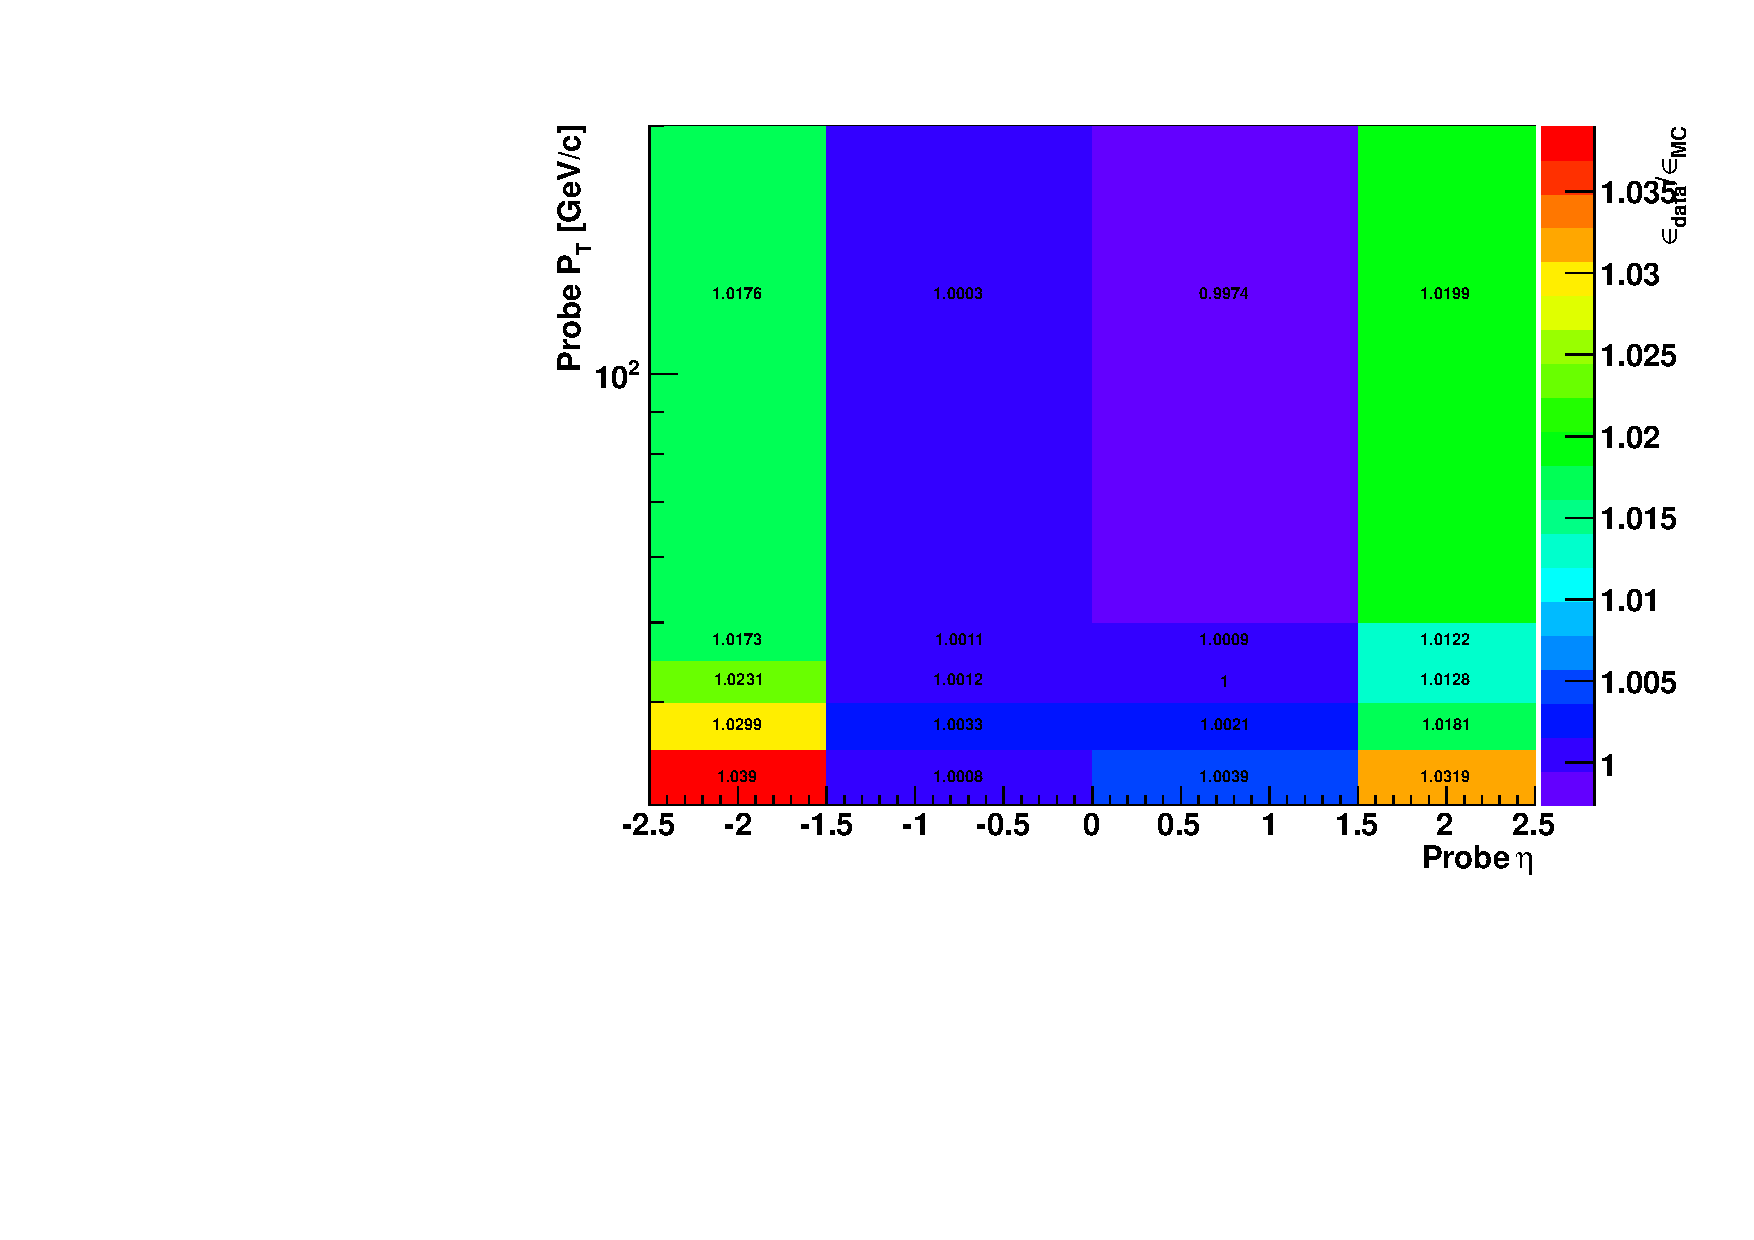
\includegraphics[width=0.32\textwidth]{plots/eleEffReco_scaleFactor.pdf}
  }
    \subfigure[]{
    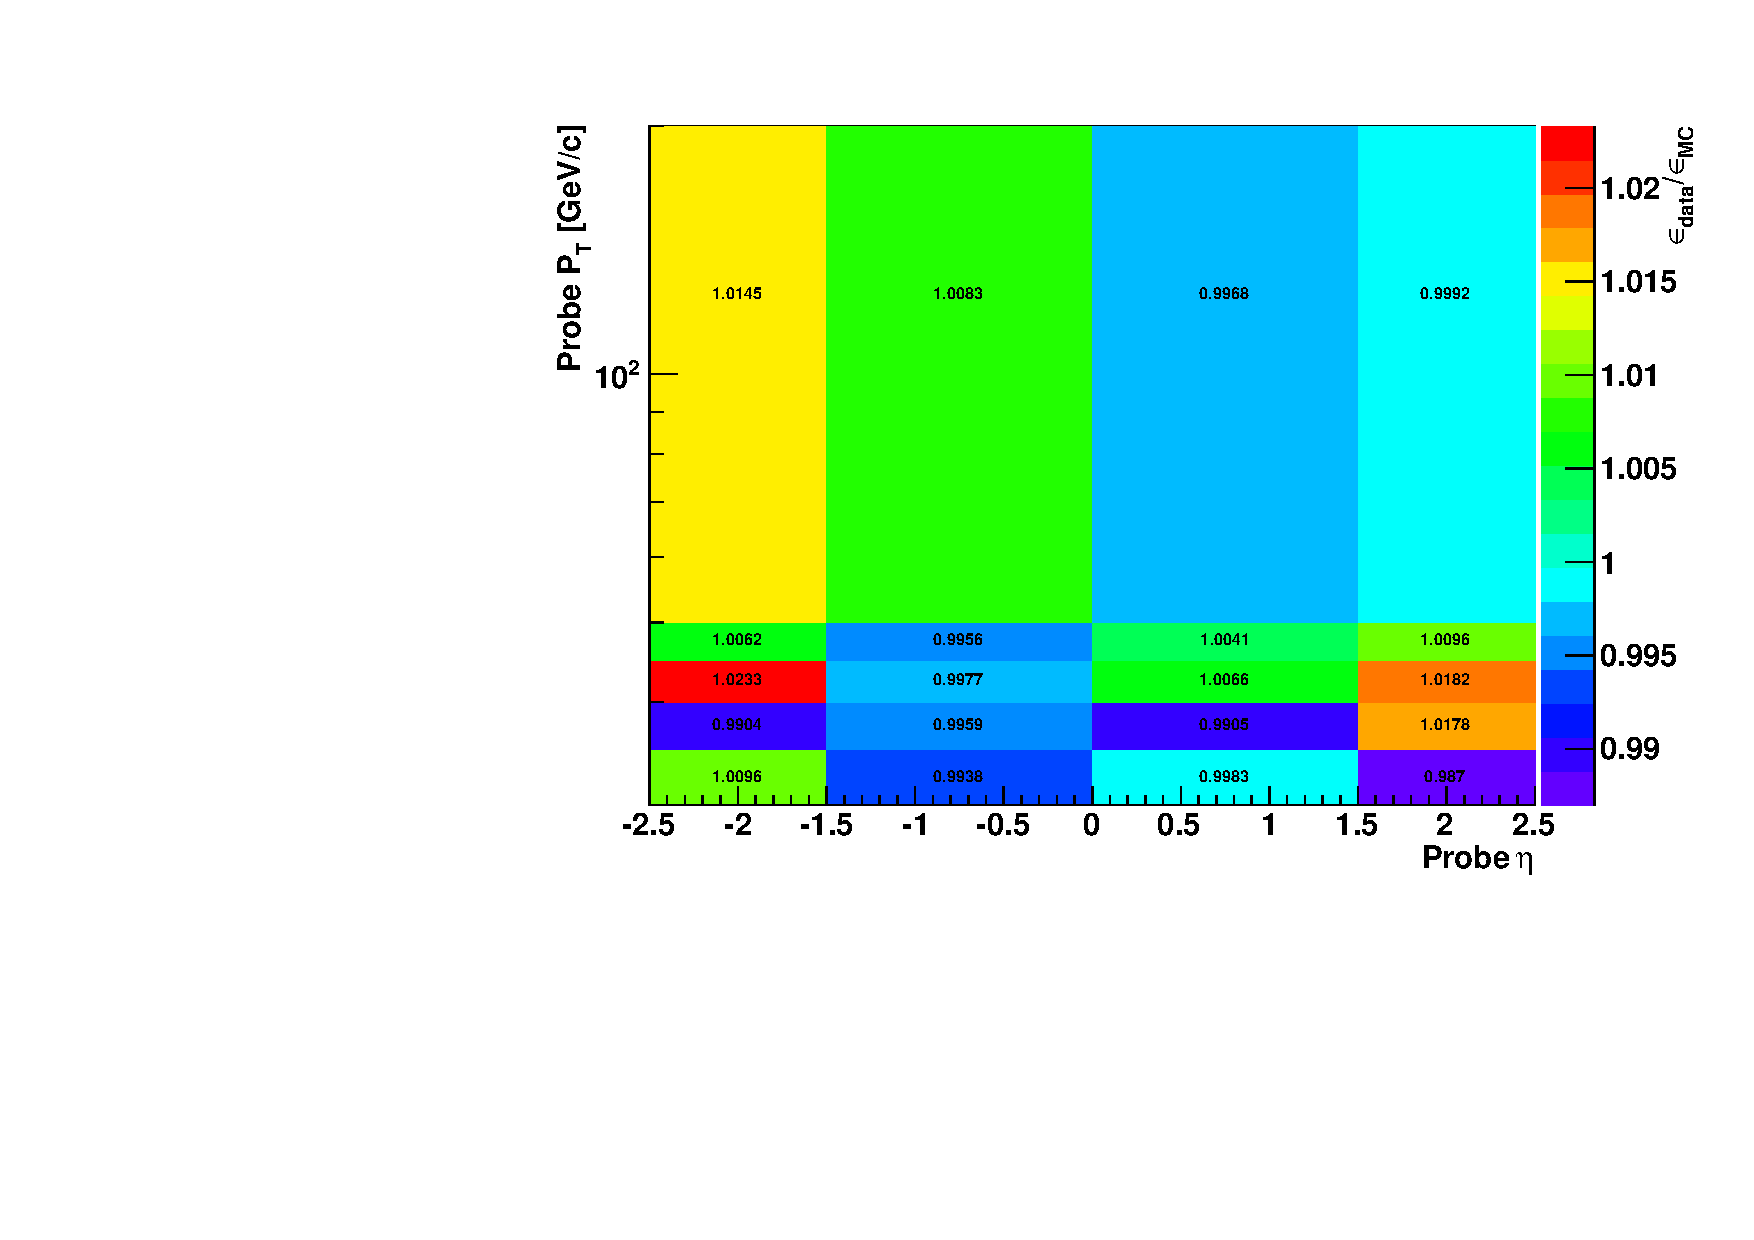
\includegraphics[width=0.32\textwidth]{plots/eleEffIso_scaleFactor.pdf}
  }
  \subfigure[]{
    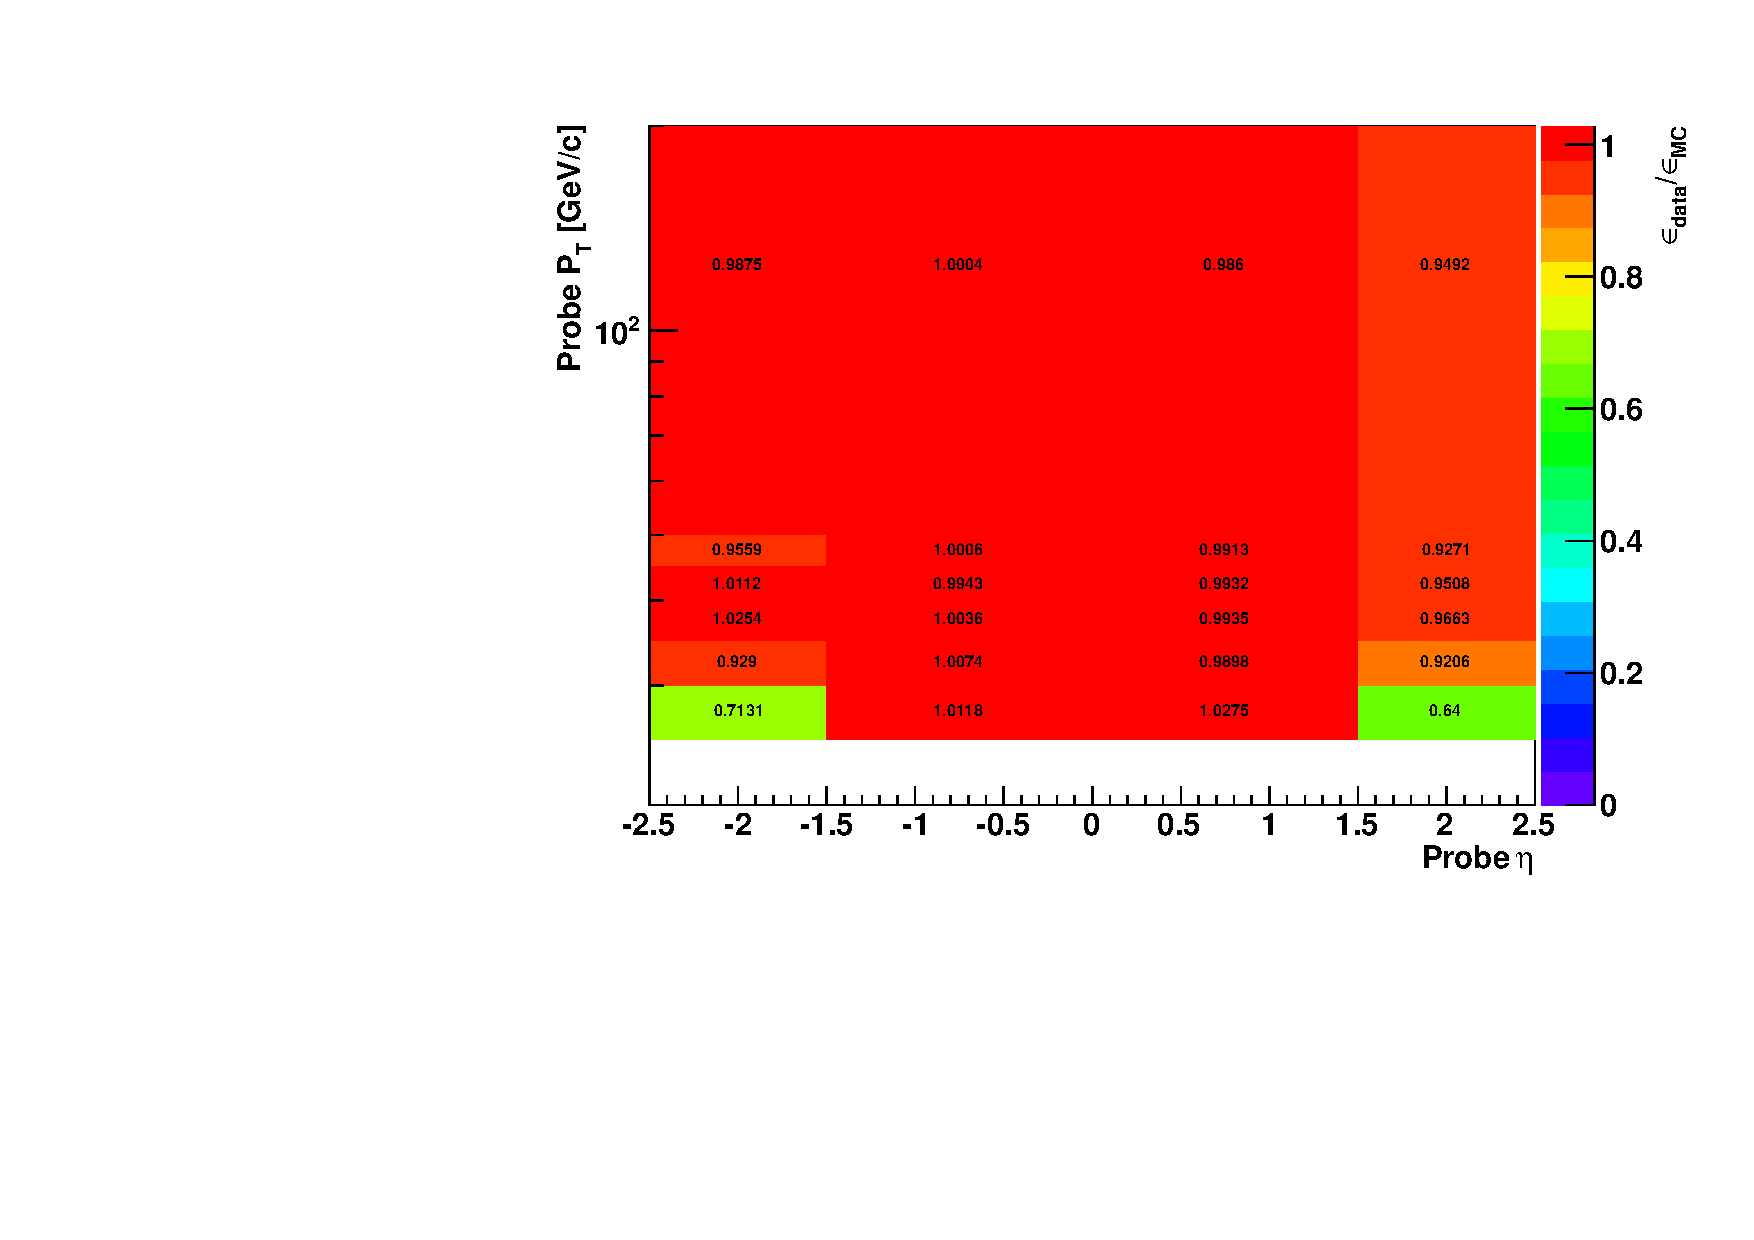
\includegraphics[width=0.32\textwidth]{plots/eleEffHLT_scaleFactor.pdf}
  }
    \caption{Electron efficiency data/MC scale factors for super-cluster to reconstructed electrons $\epsilon_{\textnormal{Reco}}$ (a), reconstructed to selected electrons $\epsilon_{\textnormal{Id}}$ (b) and selected to HLT electrons
      $\epsilon_{\textnormal{HLT}}$ (c).}
    \label{fig:eleEff}
  \end{center}
\end{figure}

\subsection{Muon efficiencies}\label{subsec:EffMu}

In the muon case, the reconstruction efficiency $\epsilon_{\textnormal{Reco}}$ describes the ability to reconstruct a Particle Flow muon starting with
a particle track and can be assumed to be one \cite{MUONPAS}. The identification efficiency $\epsilon_{\textnormal{Id}}$ gives an estimate for a
reconstructed muon to pass the offline selection criteria. It can be computed for both data and simulation and thus a scale factor being
the ratio of the two efficiencies is derived. Finally, the trigger efficiency $\epsilon_{\textnormal{HLT}}$  is the fraction of selected muons
fulfilling the HLT requirements. Since for the 2012 data a single muon trigger is used both in data and MC, a scale factor can be
computed for the HLT efficiency as well. The efficiency measurement is binned both in $\pt$ and $\eta$ of the probe muon covering the
relevant intervals (30, 35, 40, 45, 50, 200)\GeVc in $\pt$ and (-2.1, -1.5, -1.0, -0.5, 0.0, 0.5, 1.0, 1.5, 2.1) in $\eta$. The resulting selection
and trigger efficiencies and scale factors are summarized in table~\ref{tab:muonEff}. Figure~\ref{fig:muonEff} shows the data/MC scale factors
for the muon identification (a) and trigger (b).

\begin{table}[htb]
\centering 
\scalebox{0.75}{
  \begin{tabular}{|c|c|c|c|c|c|c|c|c|c|}
  \hline
  $p_{\textnormal{T,min}}$ & $p_{\textnormal{T,max}}$ & $\eta_{\textnormal{min}}$ & $\eta_{\textnormal{max}}$ & $\epsilon_{\textnormal{ID,data}}$ & $\epsilon_{\textnormal{ID,mc}}$ & $\textnormal{SF}_{\textnormal{ID}}$ & $\epsilon_{\textnormal{HLT,data}}$ & $\epsilon_{\textnormal{HLT,mc}}$ & $\textnormal{SF}_{\textnormal{HLT}}$ \\
  $[\GeVc]$         & $[\GeVc]$         &                     &                     &                            &                          &                                &                            &                           &                                \\
  \hline
  \hline
  30	& 35	& -2.1	& -1.5	& 0.930$\pm$0.004	& 0.928$\pm$0.006	& 1.002$\pm$0.008	& 0.787$\pm$0.006	& 0.737$\pm$0.010	& 1.067$\pm$0.017\\
  30	& 35	& -1.5	& -1	& 0.971$\pm$0.000	& 0.953$\pm$0.005	& 1.018$\pm$0.006	& 0.811$\pm$0.006	& 0.753$\pm$0.010	& 1.077$\pm$0.017\\
  30	& 35	& -1	& -0.5	& 0.931$\pm$0.004	& 0.946$\pm$0.006	& 0.983$\pm$0.007	& 0.895$\pm$0.004	& 0.852$\pm$0.008	& 1.051$\pm$0.011\\
  30	& 35	& -0.5	& 0	& 0.921$\pm$0.004	& 0.936$\pm$0.005	& 0.984$\pm$0.007	& 0.889$\pm$0.004	& 0.851$\pm$0.007	& 1.045$\pm$0.010\\
  30	& 35	& 0	& 0.5	& 0.929$\pm$0.004	& 0.945$\pm$0.005	& 0.983$\pm$0.006	& 0.903$\pm$0.004	& 0.861$\pm$0.007	& 1.049$\pm$0.010\\
  30	& 35	& 0.5	& 1	& 0.929$\pm$0.004	& 0.942$\pm$0.006	& 0.986$\pm$0.007	& 0.887$\pm$0.005	& 0.844$\pm$0.008	& 1.051$\pm$0.011\\
  30	& 35	& 1	& 1.5	& 0.940$\pm$0.004	& 0.943$\pm$0.003	& 0.996$\pm$0.006	& 0.787$\pm$0.006	& 0.764$\pm$0.010	& 1.031$\pm$0.015\\
  30	& 35	& 1.5	& 2.1	& 0.933$\pm$0.004	& 0.938$\pm$0.006	& 0.995$\pm$0.008	& 0.822$\pm$0.006	& 0.775$\pm$0.010	& 1.061$\pm$0.015\\
  35	& 40	& -2.1	& -1.5	& 0.929$\pm$0.003	& 0.939$\pm$0.005	& 0.989$\pm$0.007	& 0.793$\pm$0.005	& 0.770$\pm$0.008	& 1.030$\pm$0.013\\
  35	& 40	& -1.5	& -1	& 0.942$\pm$0.003	& 0.950$\pm$0.004	& 0.992$\pm$0.006	& 0.822$\pm$0.005	& 0.775$\pm$0.008	& 1.060$\pm$0.013\\
  35	& 40	& -1	& -0.5	& 0.940$\pm$0.003	& 0.947$\pm$0.029	& 0.993$\pm$0.031	& 0.901$\pm$0.003	& 0.867$\pm$0.006	& 1.039$\pm$0.008\\
  35	& 40	& -0.5	& 0	& 0.928$\pm$0.003	& 0.944$\pm$0.004	& 0.983$\pm$0.005	& 0.911$\pm$0.003	& 0.883$\pm$0.005	& 1.032$\pm$0.007\\
  35	& 40	& 0	& 0.5	& 0.928$\pm$0.003	& 0.943$\pm$0.009	& 0.985$\pm$0.010	& 0.913$\pm$0.003	& 0.871$\pm$0.005	& 1.049$\pm$0.007\\
  35	& 40	& 0.5	& 1	& 0.937$\pm$0.003	& 0.948$\pm$0.004	& 0.988$\pm$0.005	& 0.908$\pm$0.003	& 0.874$\pm$0.006	& 1.038$\pm$0.008\\
  35	& 40	& 1	& 1.5	& 0.947$\pm$0.003	& 0.947$\pm$0.005	& 1.000$\pm$0.006	& 0.803$\pm$0.005	& 0.762$\pm$0.008	& 1.054$\pm$0.013\\
  35	& 40	& 1.5	& 2.1	& 0.941$\pm$0.003	& 0.941$\pm$0.005	& 1.000$\pm$0.006	& 0.829$\pm$0.005	& 0.790$\pm$0.008	& 1.050$\pm$0.012\\
  40	& 45	& -2.1	& -1.5	& 0.956$\pm$0.005	& 0.949$\pm$0.003	& 1.007$\pm$0.006	& 0.808$\pm$0.005	& 0.769$\pm$0.007	& 1.052$\pm$0.012\\
  40	& 45	& -1.5	& -1	& 0.957$\pm$0.004	& 0.967$\pm$0.003	& 0.990$\pm$0.005	& 0.840$\pm$0.004	& 0.793$\pm$0.006	& 1.060$\pm$0.010\\
  40	& 45	& -1	& -0.5	& 0.947$\pm$0.002	& 0.955$\pm$0.003	& 0.991$\pm$0.004	& 0.913$\pm$0.003	& 0.880$\pm$0.005	& 1.037$\pm$0.006\\
  40	& 45	& -0.5	& 0	& 0.936$\pm$0.002	& 0.950$\pm$0.003	& 0.985$\pm$0.004	& 0.924$\pm$0.003	& 0.901$\pm$0.004	& 1.026$\pm$0.006\\
  40	& 45	& 0	& 0.5	& 0.936$\pm$0.002	& 0.947$\pm$0.011	& 0.988$\pm$0.012	& 0.927$\pm$0.003	& 0.897$\pm$0.004	& 1.033$\pm$0.006\\
  40	& 45	& 0.5	& 1	& 0.948$\pm$0.002	& 0.965$\pm$0.004	& 0.983$\pm$0.005	& 0.914$\pm$0.003	& 0.889$\pm$0.005	& 1.028$\pm$0.006\\
  40	& 45	& 1	& 1.5	& 0.951$\pm$0.002	& 0.964$\pm$0.006	& 0.987$\pm$0.007	& 0.810$\pm$0.004	& 0.795$\pm$0.006	& 1.019$\pm$0.010\\
  40	& 45	& 1.5	& 2.1	& 0.956$\pm$0.025	& 0.955$\pm$0.003	& 1.001$\pm$0.026	& 0.838$\pm$0.004	& 0.794$\pm$0.007	& 1.056$\pm$0.011\\
  45	& 50	& -2.1	& -1.5	& 0.944$\pm$0.003	& 0.952$\pm$0.004	& 0.991$\pm$0.006	& 0.804$\pm$0.006	& 0.796$\pm$0.009	& 1.010$\pm$0.013\\
  45	& 50	& -1.5	& -1	& 0.962$\pm$0.003	& 0.961$\pm$0.004	& 1.001$\pm$0.005	& 0.829$\pm$0.005	& 0.806$\pm$0.008	& 1.029$\pm$0.012\\
  45	& 50	& -1	& -0.5	& 0.954$\pm$0.003	& 0.955$\pm$0.004	& 0.998$\pm$0.005	& 0.924$\pm$0.003	& 0.896$\pm$0.006	& 1.031$\pm$0.007\\
  45	& 50	& -0.5	& 0	& 0.942$\pm$0.003	& 0.964$\pm$0.003	& 0.978$\pm$0.004	& 0.930$\pm$0.003	& 0.920$\pm$0.005	& 1.011$\pm$0.006\\
  45	& 50	& 0	& 0.5	& 0.946$\pm$0.003	& 0.953$\pm$0.004	& 0.993$\pm$0.005	& 0.935$\pm$0.003	& 0.917$\pm$0.005	& 1.020$\pm$0.007\\
  45	& 50	& 0.5	& 1	& 0.953$\pm$0.014	& 0.958$\pm$0.003	& 0.994$\pm$0.015	& 0.914$\pm$0.004	& 0.896$\pm$0.006	& 1.020$\pm$0.007\\
  45	& 50	& 1	& 1.5	& 0.953$\pm$0.020	& 0.962$\pm$0.004	& 0.991$\pm$0.021	& 0.822$\pm$0.005	& 0.811$\pm$0.008	& 1.014$\pm$0.012\\
  45	& 50	& 1.5	& 2.1	& 0.958$\pm$0.003	& 0.969$\pm$0.002	& 0.988$\pm$0.004	& 0.844$\pm$0.005	& 0.800$\pm$0.008	& 1.055$\pm$0.013\\
  50	& 200	& -2.1	& -1.5	& 0.952$\pm$0.006	& 0.967$\pm$0.005	& 0.985$\pm$0.008	& 0.822$\pm$0.006	& 0.809$\pm$0.009	& 1.016$\pm$0.014\\
  50	& 200	& -1.5	& -1	& 0.965$\pm$0.020	& 0.968$\pm$0.004	& 0.996$\pm$0.022	& 0.840$\pm$0.005	& 0.836$\pm$0.008	& 1.005$\pm$0.011\\
  50	& 200	& -1	& -0.5	& 0.962$\pm$0.021	& 0.963$\pm$0.004	& 1.000$\pm$0.023	& 0.921$\pm$0.004	& 0.926$\pm$0.005	& 0.995$\pm$0.007\\
  50	& 200	& -0.5	& 0	& 0.962$\pm$0.005	& 0.962$\pm$0.004	& 1.000$\pm$0.007	& 0.938$\pm$0.003	& 0.934$\pm$0.005       & 1.004$\pm$0.006\\
  50	& 200	& 0	& 0.5	& 0.940$\pm$0.012	& 0.961$\pm$0.004	& 0.978$\pm$0.013	& 0.937$\pm$0.003	& 0.934$\pm$0.005	& 1.004$\pm$0.006\\
  50	& 200	& 0.5	& 1	& 0.971$\pm$0.005	& 0.963$\pm$0.004	& 1.009$\pm$0.007	& 0.924$\pm$0.003	& 0.916$\pm$0.005	& 1.009$\pm$0.007\\
  50	& 200	& 1	& 1.5	& 0.963$\pm$0.005	& 0.954$\pm$0.005	& 1.010$\pm$0.008	& 0.812$\pm$0.006	& 0.833$\pm$0.008	& 0.975$\pm$0.012\\
  50	& 200	& 1.5	& 2.1	& 0.964$\pm$0.005	& 0.958$\pm$0.005	& 1.006$\pm$0.008	& 0.845$\pm$0.006	& 0.824$\pm$0.009	& 1.026$\pm$0.013\\
  \hline
  \end{tabular}}
\caption{Muon selection and HLT efficiency for data and MC and corresponding scale factors (SF). The errors are statistical only.} 
\label{tab:muonEff} 
\end{table}

\begin{figure}[t]
  \begin{center}
    \subfigure[]{
    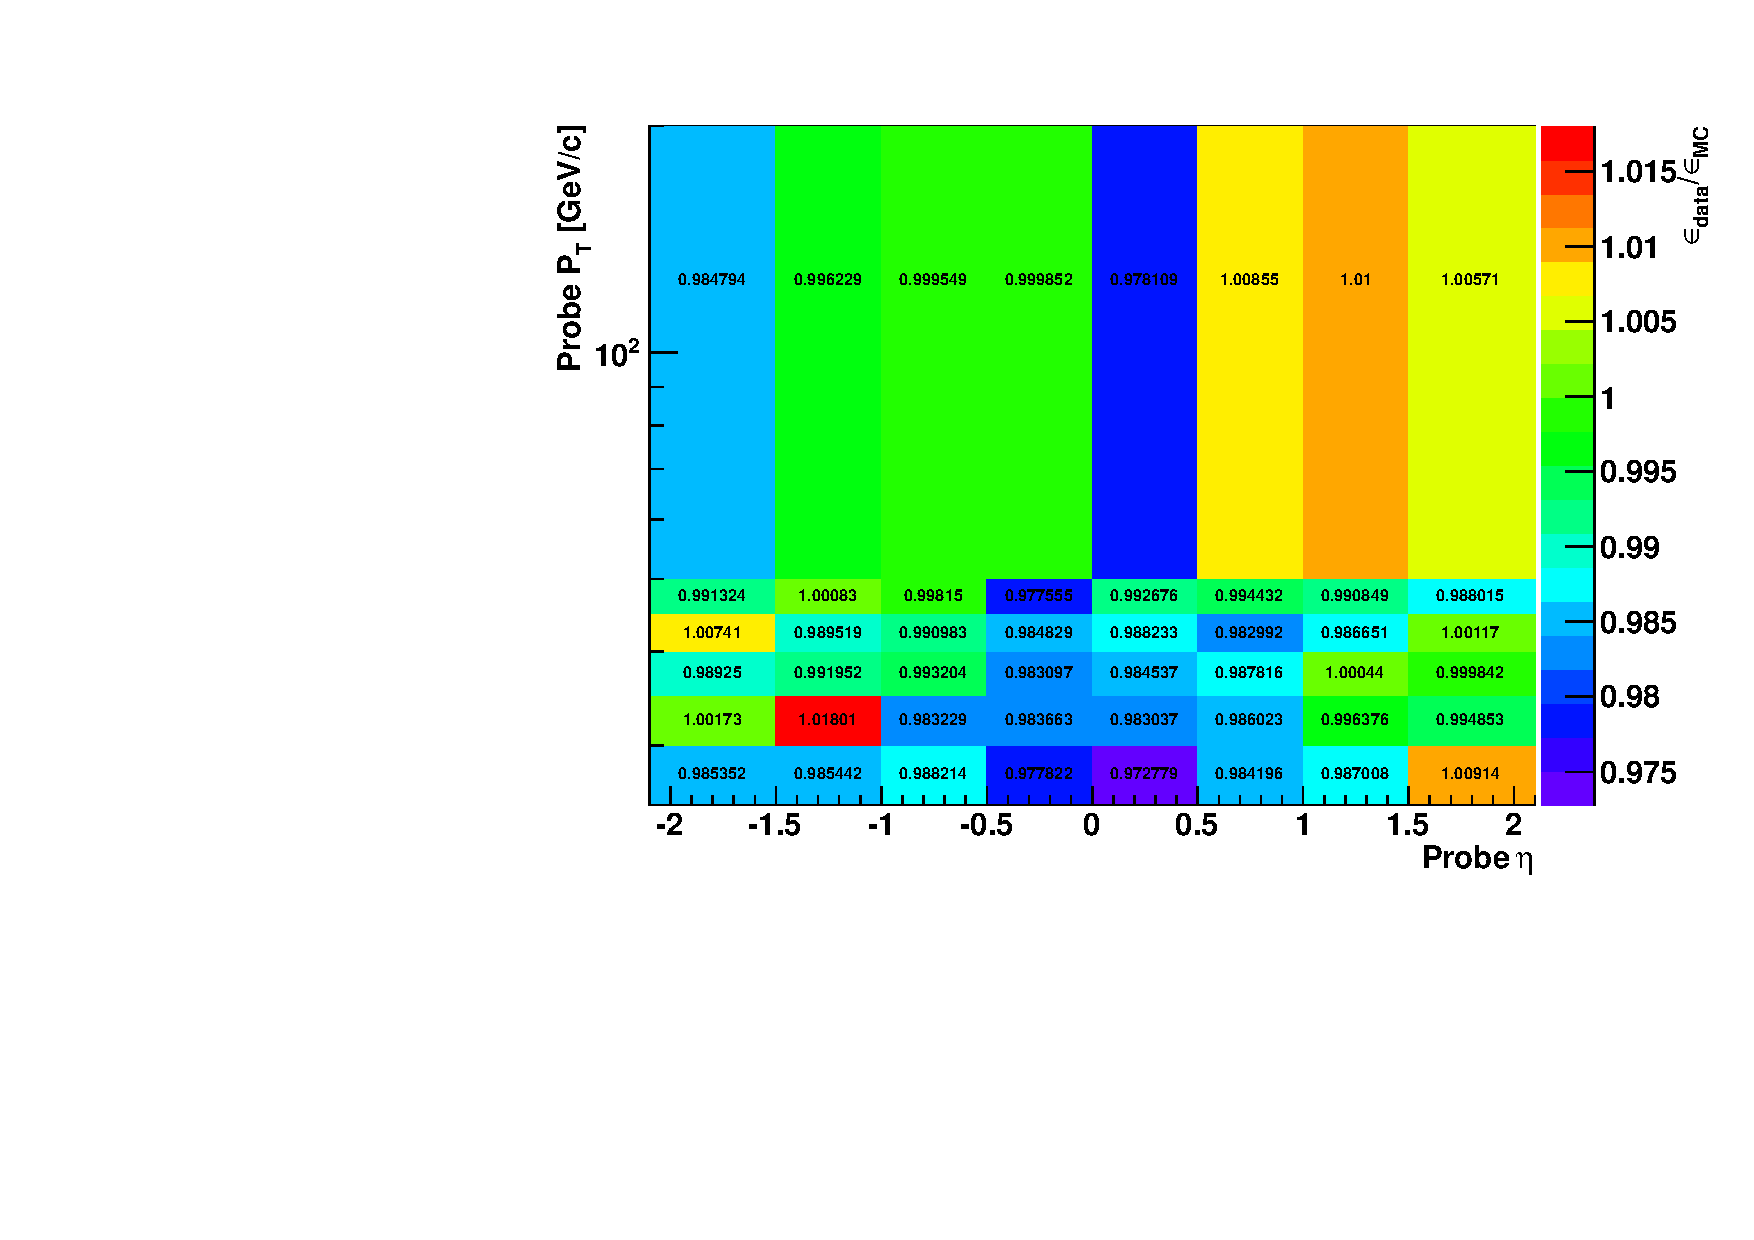
\includegraphics[width=0.47\textwidth]{plots/muEffIso_scaleFactor.pdf}
  }
  \subfigure[]{
    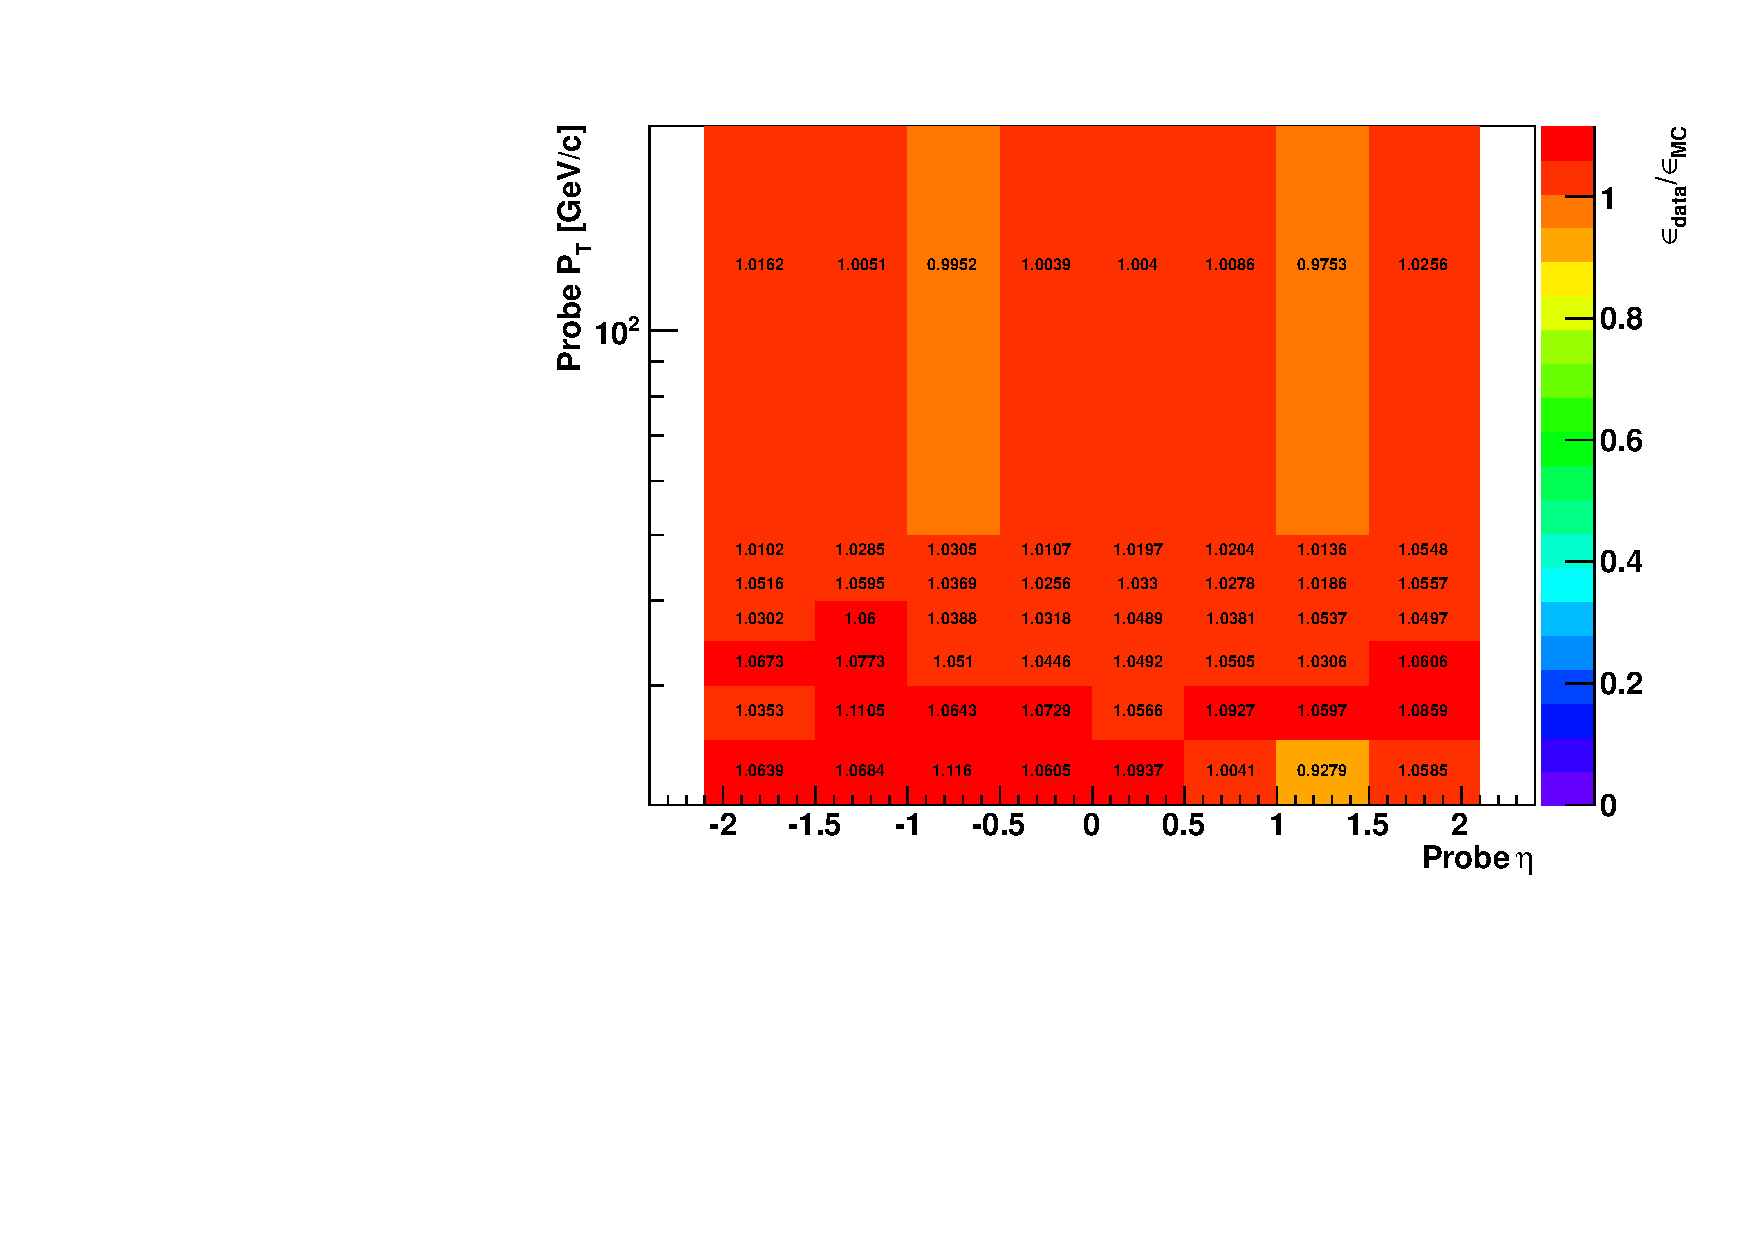
\includegraphics[width=0.47\textwidth]{plots/muEffHLT_scaleFactor.pdf}
  }
    \caption{Muon efficiency data/MC scale factors for reconstructed to selected muons $\epsilon_{\textnormal{Id}}$ (a) and for selected to HLT muons
      $\epsilon_{\textnormal{HLT}}$ (b).}
    \label{fig:muonEff}
  \end{center}
\end{figure}